\documentclass{article}

\usepackage{tikz} 
\usetikzlibrary{automata, positioning, arrows} 

\usepackage{amsthm}
\usepackage{amsfonts}
\usepackage{amsmath}
\usepackage{amssymb}
\usepackage{fullpage}
\usepackage{color}
\usepackage{parskip}
\usepackage{hyperref}
  \hypersetup{
    colorlinks = true,
    urlcolor = blue,
    linkcolor= blue,
    citecolor= blue,
    filecolor= blue,
    }
    
\usepackage{listings}
\usepackage[utf8]{inputenc}                                                    
\usepackage[T1]{fontenc}                                                       

\definecolor{dkgreen}{rgb}{0,0.6,0}
\definecolor{gray}{rgb}{0.5,0.5,0.5}
\definecolor{mauve}{rgb}{0.58,0,0.82}

\lstset{frame=tb,
  language=haskell,
  aboveskip=3mm,
  belowskip=3mm,
  showstringspaces=false,
  columns=flexible,
  basicstyle={\small\ttfamily},
  numbers=none,
  numberstyle=\tiny\color{gray},
  keywordstyle=\color{blue},
  commentstyle=\color{dkgreen},
  stringstyle=\color{mauve},
  breaklines=true,
  breakatwhitespace=true,
  tabsize=3
}

\newtheoremstyle{theorem}
  {\topsep}{\topsep}{\itshape\/}{0pt}{\bfseries}{.}{5pt plus 1pt minus 1pt}{}
\theoremstyle{theorem} 
   \newtheorem{theorem}{Theorem}[section]
   \newtheorem{corollary}[theorem]{Corollary}
   \newtheorem{lemma}[theorem]{Lemma}
   \newtheorem{proposition}[theorem]{Proposition}
\theoremstyle{definition}
   \newtheorem{definition}[theorem]{Definition}
   \newtheorem{example}[theorem]{Example}
\theoremstyle{remark}    
  \newtheorem{remark}[theorem]{Remark}

\setcounter{tocdepth}{3}
\setcounter{secnumdepth}{3}

\title{CPSC-354 Report}
\author{Jonathan Karam \\ Chapman University}

\date{\today} 

\begin{document}

\maketitle

\begin{abstract}
This report is a collection of notes, discussions, and homework solutions for CPSC 354. 
Homework 1 discusses the MIU puzzle and proves why \texttt{MI} cannot become \texttt{MU}. 
Homework 2 introduces abstract rewriting systems (ARS), includes TikZ diagrams, and classifies systems by termination, confluence, and unique normal forms. 
Homework 3 studies a rewriting system over $\{a,b\}$ and explores its equivalence classes and termination.
Homework 4 proves termination of two classic algorithms using measure functions.
Homework 5 evaluates a small $\lambda$-calculus ``workout'' using $\alpha$- and $\beta$-rules, with notes connecting these ideas to modern languages.
\end{abstract}

\tableofcontents

\section{Introduction}
This report documents my learning week by week. 
Each section includes my notes and discussions of the lecture topics, followed by my homework solutions.
The purpose is to show understanding, practice writing in \LaTeX{}, and explain the material in my own words.

\section{Week 1: The MIU Puzzle}

\subsection{Notes and Discussion}
The first week introduced the MIU puzzle, created by Douglas Hofstadter. 
It is a formal system that begins with the word \texttt{MI} and has four rules. 
The puzzle asks whether it is possible to reach \texttt{MU}. 
This is important because it shows how formal systems can be analyzed with invariants, a key concept in logic and computer science.

\subsection{Homework}
\textbf{Rules:}
\begin{enumerate}
  \item If a string ends with \texttt{I}, add a \texttt{U}.
  \item If a string starts with \texttt{M}, double the part after \texttt{M}.
  \item Replace \texttt{III} with \texttt{U}.
  \item Remove \texttt{UU}.
\end{enumerate}

\textbf{Why \texttt{MI} cannot become \texttt{MU}:}  
Let $\#I(w)$ be the number of \texttt{I}'s in $w$. Initially $\#I(\texttt{MI})=1$. 
Each rule preserves $\#I(w) \pmod{3}$:
\begin{itemize}
  \item Rule 1: no effect.
  \item Rule 2: doubles the count, $1 \mapsto 2$, never $0 \pmod 3$.
  \item Rule 3: subtracts 3, same remainder.
  \item Rule 4: no effect.
\end{itemize}
Thus $\#I(w) \pmod{3}$ is invariant. Since \texttt{MU} has $\#I=0$, it cannot be reached.

\textbf{Deeper explanation:}  
The invariant argument proves that all reachable words have I-count $\equiv 1$ or $2 \pmod{3}$, never 0.  
The first letter $M$ never disappears, so all reachable words start with $M$.  
Another way: define a homomorphism $h(M)=0, h(U)=0, h(I)=1 \pmod 3$. 
Every rule preserves $h$, so $h(\texttt{MI})=1$ and $h(\texttt{MU})=0$. Contradiction.  

\section{Week 2: Abstract Rewriting Systems}

\subsection{Notes and Discussion}
This week focused on abstract rewriting systems. 
An ARS consists of a set $A$ and a relation $R$. 
We ask whether rewriting always stops (termination), whether different rewrite paths can rejoin (confluence), and whether elements end up in unique normal forms.

\subsection{Homework}
\emph{Same problem statement as before:} draw each ARS and decide termination, confluence, and whether the system has \emph{unique normal forms for all elements} (UN-for-all).

\subsubsection*{Examples (drawings unchanged)}
\begin{tikzpicture}
  % Example 1
\end{tikzpicture}

\textbf{1: $A=\{\}, R=\{\}$} (empty system)

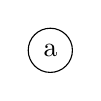
\begin{tikzpicture}
  \node[draw,circle] (a) at (0,0) {a};
\end{tikzpicture}

\textbf{2: $A=\{a\}, R=\{\}$}

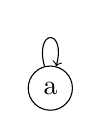
\begin{tikzpicture}
  \node[draw,circle] (a) at (0,0) {a};
  \draw[->] (a) to[loop above] (a);
\end{tikzpicture}

\textbf{3: $A=\{a\}, R=\{(a,a)\}$}

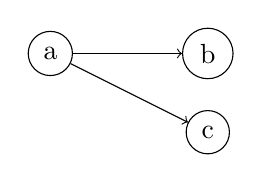
\begin{tikzpicture}
  \node[draw,circle] (a) at (0,0) {a};
  \node[draw,circle] (b) at (2,0) {b};
  \node[draw,circle] (c) at (2,-1) {c};
  \draw[->] (a) -- (b);
  \draw[->] (a) -- (c);
\end{tikzpicture}

\textbf{4: $A=\{a,b,c\}, R=\{(a,b),(a,c)\}$}

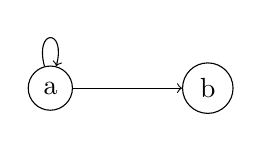
\begin{tikzpicture}
  \node[draw,circle] (a) at (0,0) {a};
  \node[draw,circle] (b) at (2,0) {b};
  \draw[->] (a) to[loop above] (a);
  \draw[->] (a) -- (b);
\end{tikzpicture}

\textbf{5: $A=\{a,b\}, R=\{(a,a),(a,b)\}$}

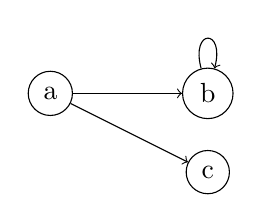
\begin{tikzpicture}
  \node[draw,circle] (a) at (0,0) {a};
  \node[draw,circle] (b) at (2,0) {b};
  \node[draw,circle] (c) at (2,-1) {c};
  \draw[->] (a) -- (b);
  \draw[->] (a) -- (c);
  \draw[->] (b) to[loop above] (b);
\end{tikzpicture}

\textbf{6: $A=\{a,b,c\}, R=\{(a,b),(b,b),(a,c)\}$}

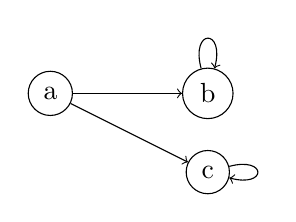
\begin{tikzpicture}
  \node[draw,circle] (a) at (0,0) {a};
  \node[draw,circle] (b) at (2,0) {b};
  \node[draw,circle] (c) at (2,-1) {c};
  \draw[->] (a) -- (b);
  \draw[->] (a) -- (c);
  \draw[->] (b) to[loop above] (b);
  \draw[->] (c) to[loop right] (c);
\end{tikzpicture}

\textbf{7: $A=\{a,b,c\}, R=\{(a,b),(b,b),(a,c),(c,c)\}$}

\subsubsection*{Classification (solutions rewritten)}
We now use \textbf{UN-for-all}: every element must have a (unique) normal form.

\[
\begin{array}{c|c|c|c|l}
\text{ARS} & \text{Terminating} & \text{Confluent} & \text{UN-for-all} & \text{Why} \\\hline
1 & \text{Yes} & \text{Yes} & \text{Yes} & \text{Nothing rewrites (vacuous).} \\
2 & \text{Yes} & \text{Yes} & \text{Yes} & a \text{ is already normal and unique.} \\
3 & \text{No} & \text{Yes} & \text{No}  & a \to a \text{ forever; } a \text{ has no NF.} \\
4 & \text{Yes} & \text{No}  & \text{No}  & a\to b,\,a\to c \text{ (two distinct NFs).} \\
5 & \text{No} & \text{Yes} & \text{Yes} & a\to b,\; b \text{ normal; both end at } b. \\
6 & \text{No} & \text{No}  & \text{No}  & b \text{ loops; } a\to c \text{ NF, not joinable with } b. \\
7 & \text{No} & \text{No}  & \text{No}  & b,c \text{ loop; no element has an NF.} \\
\end{array}
\]

\paragraph{Remarks.}
\begin{itemize}
  \item Non-termination alone does not rule out UN-for-all (see 5), but any element without an NF breaks it (3,6,7).
  \item In terminating ARSs, confluence $\Rightarrow$ UN-for-all (every element reaches a unique NF).
  \item Item 4 is the canonical “diamond failure”: two different normal forms reachable from the same source.
\end{itemize}

\section{Week 3: Strings over \{a,b\}}

\subsection{Notes and Discussion}
We studied rewriting rules over alphabet $\{a,b\}$. 
This shows how simple systems can classify strings into equivalence classes. 
We also saw how orienting rules one way can make a system terminating without changing equivalence.

\subsection{Homework 3}
\textbf{Exercise 5 rules:}
\[
ab \to ba,\quad ba \to ab,\quad aa \to \varepsilon,\quad b \to \varepsilon
\]

Examples: \texttt{abba} $\to$ \texttt{aa} $\to$ $\varepsilon$.  
\texttt{bababa} $\to$ \texttt{aaa} $\to$ \texttt{a}.  

Not terminating because swaps loop.  
Equivalence classes: even number of $a$’s $\to \varepsilon$, odd $\to a$.  
Normal forms: $\varepsilon, a$.  
Fix: orient $ba \to ab$ only.  

\textbf{Exercise 5b rules:}
\[
ab \leftrightarrow ba,\quad aa \to a,\quad b \to \varepsilon
\]

Examples: \texttt{abba} $\to$ \texttt{a}. \texttt{bababa} $\to$ \texttt{a}.  

Equivalence: all $b$ vanish, runs of $a$ collapse to one $a$.  
Classes: $\{\varepsilon,a\}$.  
Fix: orient swaps, keep $aa \to a$ and $b \to \varepsilon$.  

\section{Week 4: Measure Functions and Termination}

\subsection{Notes and Discussion}
This week we looked at \emph{measure functions} to prove that algorithms terminate.
A measure maps the state of a computation to a value in a well-founded set (usually the natural numbers) and must
\emph{strictly decrease} with every loop iteration or recursive call. Because there are no infinite descending chains in a well-founded set, the computation must eventually stop.

\textbf{Scope note:} For the homework we include only what is required: define a measure and show it strictly decreases (hence termination).

\paragraph{Class notes — invariant proof that Euclid returns $\gcd$.}
\begin{itemize}
  \item \textbf{Key fact.} $\gcd(a,b)=\gcd\!\big(b,\,a-qb\big)$ for any integer $q$.
  \item \textbf{Update.} Writing $a=qb+r$ with $r=a\bmod b$, the step $(a,b)\mapsto(b,r)$ keeps the gcd unchanged.
  \item \textbf{Invariant.} Before each loop test: $\gcd(a,b)=\gcd(a_0,b_0)$.
  \item \textbf{End.} When $b=0$, $\gcd(a_0,b_0)=\gcd(a,0)=|a|$, the returned value.
\end{itemize}

\subsection{Homework 4}

\subsubsection*{HW 4.1}
\textbf{Problem.} Consider:
\begin{lstlisting}[language=Python]
while b != 0:
    temp = b
    b = a % b
    a = temp
return a
\end{lstlisting}
Under which conditions does this algorithm always terminate? Find a measure function and prove termination.

\medskip
\textbf{Answer.}  
This is the classical Euclidean algorithm for $\gcd(a,b)$. It always terminates provided
\[
a,b \in \mathbb{Z}\quad\text{and}\quad b \ge 0,
\]
and we interpret \texttt{\%} as the mathematical remainder with $0 \le a \bmod b < b$ for $b>0$. (If inputs may be negative, replace them once by $|a|,|b|$; this preserves $\gcd$ and satisfies the condition.)

\paragraph{Measure function.}
Let the program state be the pair $(a,b)$ with $b \ge 0$. Define
\[
\mu(a,b) \;=\; b \in \mathbb{N}.
\]

\paragraph{Strict decrease.}
In an iteration with $b>0$ we set $b' = a \bmod b$. By definition of remainder,
\[
0 \le b' < b.
\]
Therefore $\mu(a',b') = b' < b = \mu(a,b)$. Hence $\mu$ strictly decreases on every loop step.

\paragraph{Well-foundedness and termination.}
$\mu$ maps states to the natural numbers with the usual $<$, which is well-founded (no infinite descending chains). Because $\mu$ strictly decreases whenever the loop body executes, the loop can execute only finitely many times; eventually $b=0$ and the algorithm returns. \qed

\begin{remark}
The algorithm not only terminates; it returns $\gcd(a,b)$. This follows from the class-note invariant above and $\gcd(a,0)=|a|$.
\end{remark}

\subsubsection*{HW 4.2}
\textbf{Problem.} Consider the fragment of merge sort:
\begin{lstlisting}[language=Python]
def merge_sort(arr, left, right):
    if left >= right:
        return
    mid = (left + right) // 2
    merge_sort(arr, left, mid)
    merge_sort(arr, mid + 1, right)
    merge(arr, left, mid, right)
\end{lstlisting}
Prove that
\[
\varphi(left,right) \;=\; right - left + 1
\]
is a measure function for \texttt{merge\_sort}.

\medskip
\textbf{Answer.}
We show that every recursive call is made with a \emph{strictly smaller} measure and that the measure is bounded below by $0$.

\paragraph{Well-founded codomain.}
$\varphi(left,right)$ is a nonnegative integer whenever $left\le right$, so the codomain is $\mathbb{N}$ with the usual $<$ (well-founded).

\paragraph{Base case.}
If $left \ge right$, the function returns immediately. In this case $\varphi \le 1$, and there are no recursive calls.

\paragraph{Decrease for recursive calls.}
Assume $left < right$ and let $n = \varphi(left,right) = right-left+1 \ge 2$. With
\[
mid = \left\lfloor \frac{left+right}{2} \right\rfloor,
\]
the first recursive call is on $[left,\,mid]$ and the second on $[mid+1,\,right]$. Their measures are
\[
\varphi(left,mid) = mid - left + 1, \qquad
\varphi(mid+1,right) = right - mid.
\]
Because $left \le mid < right$, we have
\[
1 \le \varphi(left,mid) \le \left\lceil \frac{n}{2}\right\rceil < n,\qquad
1 \le \varphi(mid+1,right) \le \left\lfloor \frac{n}{2}\right\rfloor < n.
\]
Thus each recursive call receives strictly smaller measure than $n$.

\paragraph{Conclusion.}
Every chain of recursive calls strictly decreases $\varphi$ and cannot be infinite in $\mathbb{N}$. Therefore \texttt{merge\_sort} terminates. \qed

\section{Week 5: Lambda Calculus Foundations}

\subsection{Notes and Discussion}
\begin{itemize}
  \item \textbf{Self-application and computation.} Terms like $(\lambda x.\,xx)(\lambda x.\,xx)$ show that functions can take \emph{code as data}. This enables iteration/recursion encodings (fixed points) and explains why untyped $\lambda$ can express non-termination.
  \item \textbf{Where $\lambda$ shines.} Useful for building \emph{minimal cores}: interpreters, proof assistants, type checkers, compiler IRs, and reasoning about higher-order functions. It models substitution, scope, closures, and evaluation precisely.
  \item \textbf{Composition and numerals.} Church numerals encode iteration: $\mathbf{n}\,f\,x = f^{n}x$. Function composition $(f \circ g)$ corresponds to multiplying numerals: $(\mathbf{m}\circ\mathbf{n})\,f\,x = f^{mn}x$. Plain application behaves like \emph{exponentiation in reverse order}: $\mathbf{m}\,\mathbf{n} = \mathbf{n}^{\,\mathbf{m}}$ (apply $\mathbf{m}$ times), so $\mathbf{2}\,\mathbf{3}=\mathbf{9}$ and $\mathbf{3}\,\mathbf{2}=\mathbf{8}$.
  \item \textbf{Confluence (Church–Rosser).} If a term reduces to two results, there exists a common reduct. Meaning: evaluation order doesn’t affect the final normal form (when it exists). Languages borrow this idea to justify equational reasoning and optimizations.
  \item \textbf{From $\lambda$ to languages.} Add types (safety), effects (state, I/O), data types, and evaluation strategy to get modern languages. Typed $\lambda$-calculi (System~F, Hindley–Milner) underlie ML/Haskell; effect systems/monads model side effects.
  \item \textbf{Haskell links.} Purity, first-class functions, laziness (normal-order–like), algebraic data types, and type inference all line up with typed $\lambda$-calculus. Monads/Applicatives are structured ways to compose computations.
  \item \textbf{Names and $\alpha$-conversion.} Variables need not be single letters; names are irrelevant up to $\alpha$-equivalence (consistent renaming). Modern languages reflect this via lexical scope, hygienic macros, and compiler renaming to avoid capture.
  \item \textbf{The role of $\alpha$ in practice.} Compilers implement renaming and fresh-name generation to maintain scope hygiene (e.g., SSA form, macro expansion).
  \item \textbf{Termination and type systems.} Untyped $\lambda$ allows non-termination (Y-combinator). Total languages (Coq/Agda) \emph{forbid} general recursion by checking termination via structural/lexicographic and multivariate measures; complex patterns (exponential, multi-dimension decrease) are handled with well-founded orders and sized types. Downsides: proofs/measures can cost compile time (sometimes exponential).
  \item \textbf{Original intent.} Church invented $\lambda$ for the foundations of mathematics (functions as rules of calculation) and to study effective computability—leading to Church–Turing thesis.
  \item \textbf{Recursion vs loops.} Prefer recursion when structure is naturally recursive (trees, syntax, divide-and-conquer) or when immutability/purity matters. Prefer loops when iterating in-place over arrays or when tail recursion isn’t optimized.
  \item \textbf{What can/can’t be expressed.} Untyped $\lambda$ can encode any computable function (Turing complete). Exact analysis over reals (symbolic integrals) can be encoded with representations, but decidability and performance are not guaranteed; many problems are undecidable.
  \item \textbf{Meaning vs representation.} $\alpha$-equivalence shows semantics can be invariant under renaming. Suggests programs’ meaning depends on structure and binding, not surface spelling.
  \item \textbf{Infinitely long calls?} Reductions can be infinite (non-terminating), but any single step is finite. Typed total calculi restrict to well-founded recursion to rule these out.
\end{itemize}

\subsection{Homework 5: Lambda Calculus Workout}

\subsubsection*{Problem}
Evaluate (practice $\alpha$ and $\beta$ rules; match parentheses):
\[
\Big(\lambda f.\,\lambda x.\,f(f\,x)\Big)\;
\Big(\lambda f.\,\lambda x.\,f(f(f\,x))\Big).
\]

\subsubsection*{Solution}
Let
\[
\mathbf{two} \equiv \lambda f.\lambda x.\,f(fx),\qquad
\mathbf{three} \equiv \lambda f.\lambda x.\,f(f(fx)).
\]
Then
\[
\mathbf{two}\;\mathbf{three}
\;\xrightarrow{\beta}\;
\lambda x.\,\mathbf{three}\,(\mathbf{three}\,x).
\]
Compute:
\[
\mathbf{three}\,x \xrightarrow{\beta} \lambda y.\,x(x(x\,y)),
\qquad
\mathbf{three}\,(\lambda y.\,x(x(x\,y))) \xrightarrow{\beta} \lambda z.\,x^{9}z.
\]
Therefore
\[
\boxed{\lambda x.\lambda z.\,x^{9}z}
\]
which is the Church numeral $\mathbf{nine}$.

\paragraph{Swap note.}
$\mathbf{3}\,\mathbf{2}=\mathbf{8}$, not $\mathbf{9}$, because application acts like exponentiation with reversed order: $\mathbf{m}\,\mathbf{n}=\mathbf{n}^{\,\mathbf{m}}$.

\section{Conclusion}
\textbf{Week 1:} Learned about invariants and why MU is impossible.  
\textbf{Week 2:} Revisited ARS pictures and re-answered termination/confluence/UN with the UN-for-all convention.  
\textbf{Week 3:} Explored rewriting with $\{a,b\}$, equivalence classes, and how termination can be fixed.\\
\textbf{Week 4:} Used measure functions to prove termination of Euclid's algorithm and merge sort.\\
\textbf{Week 5:} Connected $\lambda$-calculus ideas (self-application, confluence, Church numerals) to modern language design and evaluated the workout.

\begin{thebibliography}{99}
\bibitem[BLA]{bla} Author, \href{https://en.wikipedia.org/wiki/LaTeX}{LaTeX Overview}, Publisher, Year.
\end{thebibliography}

\end{document}
